\section{Rational Inequalities and Applications}

\label{RationalIneq}

In this section, we solve equations and inequalities involving rational functions and explore associated application problems. Our first example showcases the critical difference in procedure between solving a rational equation and a rational inequality.

\medskip

\example{ex_ratineq}{Rational equation and inequality}{
\begin{enumerate}

\item  Solve $\dfrac{x^3-2x+1}{x-1} = \dfrac{1}{2}x-1$.

\item  Solve $\dfrac{x^3-2x+1}{x-1} \geq \dfrac{1}{2}x-1$.

\item  Use your computer or calculator to graphically check your answers to 1 and 2.

\end{enumerate}
}
{
\begin{enumerate}

\item  To solve the equation, we clear denominators

\[ \begin{array}{rclr}

\dfrac{x^3-2x+1}{x-1} & = & \dfrac{1}{2}x-1 & \\ [10pt]

\left(\dfrac{x^3-2x+1}{x-1}\right) \cdot 2(x-1) & = & \left( \dfrac{1}{2}x-1 \right) \cdot 2(x-1) & \\ [10pt]

2x^3 - 4x + 2 & = & x^2-3x+2 & \mbox{expand} \\

2x^3 -x^2 - x & = & 0 & \\

x(2x+1)(x-1) & = & 0 & \mbox{factor}\\

x & = & -\frac{1}{2}, \, 0, \, 1 & \\


\end{array}\]

Since we cleared denominators, we need to check for extraneous solutions.  Sure enough, we see that $x=1$ does not satisfy the original equation and must be discarded.  Our solutions are $x=-\frac{1}{2}$ and $x=0$.

\item  To solve the inequality, it may be tempting to begin as we did with the equation $-$ namely by multiplying both sides by the quantity $(x-1)$.  The problem is that, depending on $x$, $(x-1)$ may be positive (which doesn't affect the inequality) or $(x-1)$ could be negative (which would reverse the inequality).  Instead of working by cases, we collect all of the terms on one side of the inequality with $0$ on the other and make a sign diagram using the technique given on page \pageref{rationalsigndiagram} in Section \ref{RationalGraphs}.

\begin{align*}
\dfrac{x^3-2x+1}{x-1} & \geq \dfrac{1}{2}x-1  \\ 
\dfrac{x^3-2x+1}{x-1}  - \dfrac{1}{2} x + 1& \geq  0 \\
\dfrac{2\left(x^3-2x+1\right)-x(x-1)+1(2(x-1))}{2(x-1)} & \geq  0  \tag*{get a common denominator} \\ 
\dfrac{2x^3-x^2-x}{2x-2} & \geq  0  \tag*{expand}
\end{align*}

Viewing the left hand side as a rational function $r(x)$ we make a sign diagram.  The only value excluded from the domain of $r$ is $x=1$ which is the solution to $2x-2=0$.  The zeros of $r$ are the solutions to $2x^3-x^2-x=0$, which we have already found to be $x=0$, $x=-\frac{1}{2}$ and $x=1$, the latter was discounted as a zero because it is not in the domain.  Choosing test values in each test interval, we obtain the sign diagram in Figure \ref{fig:ratineq1}. 

\mfigure{.85}{The sign diagram for the inequality in Example \ref{ex_ratineq}}{fig:ratineq1}{figures/RationalsGraphics/RationalIneq-1}

We are interested in where $r(x) \geq 0$.  We find $r(x) > 0$, or $(+)$, on the intervals $\left(-\infty, -\frac{1}{2}\right)$, $(0,1)$ and $(1, \infty)$.  We add to these intervals the zeros of $r$, $-\frac{1}{2}$ and $0$, to get our final solution:  $\left( - \infty, -\frac{1}{2} \right] \cup [0,1) \cup (1, \infty)$.

\item  Geometrically, if we set $f(x) = \dfrac{x^3-2x+1}{x-1}$ and $g(x) = \frac{1}{2} x -1$, the solutions to $f(x)=g(x)$ are the $x$-coordinates of the points where the graphs of $y=f(x)$ and $y=g(x)$ intersect.  The solution to $f(x) \geq g(x)$ represents not only where the graphs meet, but the intervals over which the graph of $y=f(x)$ is above ($>$) the graph of $g(x)$. Entering these two functions into GeoGebra gives us Figure \ref{fig:ratineq2}. 

\mfigure[width=0.95\marginparwidth]{.7}{The initial plot of $f(x)$ and $g(x)$}{fig:ratineq2}{figures/RationalsGraphics/Rationals10}

\mfigure[width=0.95\marginparwidth]{.5}{Zooming in to find the intersection points}{fig:ratineq3}{figures/RationalsGraphics/Rationals11}

Zooming in and using the Intersect tool, we see in Figure \ref{fig:ratineq3} that the graphs cross when $x=-\frac{1}{2}$ and $x=0$.  It is clear from the calculator that the graph of $y=f(x)$ is above the graph of $y=g(x)$ on $\left(-\infty, -\frac{1}{2}\right)$ as well as on $(0,\infty)$.  According to the calculator, our solution is then $\left(-\infty, -\frac{1}{2}\right] \cup [0, \infty)$ which \textit{almost} matches the answer we found analytically.  We have to remember that $f$ is not defined at $x=1$, and, even though it isn't shown on the calculator, there is a hole in the graph of $y=f(x)$ when $x=1$ which is why $x=1$ is not part of our final answer. (There is no asymptote at $x=1$ since the graph is well behaved near $x=1$.  According to Theorem \ref{vavshole}, there  must be a hole there.)

\end{enumerate}
}  

\medskip

Next, we explore how rational equations can be used to solve some classic problems involving rates.

\medskip

\example{upstreamdownstreamex}{Calculating the speed of a river}{  Carl decides to explore the Meander River, the location of several recent Sasquatch sightings.  From camp, he canoes downstream five miles to check out a purported Sasquatch nest.  Finding nothing, he immediately turns around, retraces his route (this time travelling upstream), and returns to camp 3 hours after he left.  If Carl canoes at a rate  of 6 miles per hour in still water, how fast was the Meander River flowing on that day?
}
{
We are given information about distances, rates (speeds) and times.  The basic principle relating these quantities is: \[ \text{distance} = \text{rate} \cdot \text{time}\]  The first observation to make, however, is that the distance, rate and time given to us aren't `compatible':  the distance given is the distance for only \textit{part} of the trip,  the rate given is the speed Carl can canoe in still water, not in a flowing river, and  the time given is the duration of the \textit{entire} trip.  Ultimately, we are after the speed of the river, so let's call that $R$ measured in miles per hour to be consistent with the other rate given to us.  To get started, let's divide the trip into its two parts:  the initial trip downstream and the return trip upstream.  For the downstream trip, all we know is that the distance travelled is $5$ miles.

\[ \begin{array}{rcl}

\text{distance downstream} & = & \text{rate travelling downstream} \cdot \text{time travelling downstream} \\

5 \, \text{miles} & = & \text{rate travelling downstream} \cdot \text{time travelling downstream} \\ \end{array} \]

Since the return trip upstream followed the same route as the trip downstream, we know that the distance travelled upstream is also 5 miles.

\[ \begin{array}{rcl}

\text{distance upstream} & = & \text{rate traveling upstream} \cdot \text{time traveling upstream} \\

5 \, \text{miles} & = & \text{rate traveling upstream} \cdot \text{time traveling upstream} \\ \end{array} \]

We are told Carl can canoe at a  rate of $6$ miles per hour in still water.  How does this figure into the rates travelling upstream and downstream?  The speed the canoe travels in the river is a combination of the speed at which Carl can propel the canoe in still water, 6 miles per hour,  and the speed of the river, which we're calling $R$. When travelling downstream, the river is helping Carl along, so we \textit{add} these two speeds: 

\[ \begin{array}{rcl}

\text{rate traveling downstream} & = & \text{rate Carl propels the canoe} + \text{speed of the river} \\

 & = & 6 \frac{\text{miles}}{\text{hour}} + R \frac{\text{miles}}{\text{hour}} \\ \end{array} \]
 
 So our downstream speed is $(6+R) \frac{\text{miles}}{\text{hour}}$.  Substituting this into our `distance-rate-time' equation for the downstream part of the trip, we get:
 
 \[ \begin{array}{rcl}

5 \, \text{miles} & = & \text{rate traveling downstream} \cdot \text{time traveling downstream} \\ 

5 \, \text{miles} & = & (6+R) \frac{\text{miles}}{\text{hour}} \cdot \text{time traveling downstream} \\ 	\end{array} \]

 When travelling upstream, Carl works against the current.  Since the canoe manages to travel upstream,  the speed Carl can canoe in still water is greater than the river's speed, so we \textit{subtract} the river's speed \textit{from} Carl's canoeing speed to get:
 
 \[ \begin{array}{rcl}

\text{rate traveling upstream} & = & \text{rate Carl propels the canoe} - \text{river speed} \\

 & = & 6 \frac{\text{miles}}{\text{hour}} - R \frac{\text{miles}}{\text{hour}} \\ \end{array} \]
 
Proceeding as before, we get
 
 \[ \begin{array}{rcl}

5 \, \text{miles} & = & \text{rate traveling upstream} \cdot \text{time traveling upstream} \\ 

5 \, \text{miles} & = & (6 - R) \frac{\text{miles}}{\text{hour}} \cdot \text{time traveling upstream} \\ 	\end{array} \]
 
The last piece of information given to us is that the total trip lasted $3$ hours.  If we let $t_{\text{down}}$ denote the time of the downstream trip and $t_{\text{up}}$ the time of the upstream trip, we have:    $t_{\text{down}} + t_{\text{up}} = 3 \, \text{hours}$.  Substituting $t_{\text{down}}$ and $t_{\text{up}}$ into the `distance-rate-time' equations, we get (suppressing the units) \textit{three} equations in \textit{three} unknowns:
 \[\left\{\begin{array}{lrcl}   E1 & (6+R) \, t_{\text{down}} & = & 5 \\ E2 & (6-R) \, t_{\text{up}} & = & 5 \\ E3 & t_{\text{down}} + t_{\text{up}} & = & 3 \end{array} \right.\]

\mnote{.25}{This is an example of a \textit{system} of equations.  If you didn't encounter such creatures in high school, don't worry: you won't need to solve any systems in this course. If you're wondering if there's a general procedure for tackling such problems, you might want to check out Math 1410.}

\mnote{.15}{Although we usually discourage dividing both sides of an equation by a variable expression, we know $(6+R) \neq 0$ since otherwise we couldn't possibly multiply it by $t_{\text{down}}$ and get $5$.}

Since we are ultimately after $R$, we need to use these three equations to get at least one equation involving only $R$.  To that end, we solve $E1$ for $t_{\text{down}}$ by dividing both sides by the quantity $(6+R)$ to get $t_{\text{down}} = \dfrac{5}{6+R}$.   Similarly, we solve $E2$ for $t_{\text{up}}$ and get $t_{\text{up}} = \dfrac{5}{6-R}$. Substituting these into $E3$, we get: \[\dfrac{5}{6+R} + \dfrac{5}{6 - R} = 3.\] 
(The reader is encouraged to verify that the units in this equation are the same on both sides.  To get you started, the units on the `3' is `hours.') Clearing denominators, we get $5(6-R) + 5(6+R) = 3(6+R)(6-R)$ which reduces to  $R^2 = 16$.   We find $R = \pm 4$, and since $R$ represents the speed of the river, we choose $R = 4$.   On the day in question, the Meander River is flowing at a rate of $4$ miles per hour. 


}

\medskip

One of the important lessons to learn from Example \ref{upstreamdownstreamex} is that speeds, and more generally, rates, are additive.  As we see in our next example, the concept of rate and its associated principles can be applied to a wide variety of problems - not just `distance-rate-time' scenarios.

\medskip

\example{workex}{Calculating work rates}{  Working alone, Taylor can weed the garden in 4 hours.  If Carl helps, they can weed the garden in 3 hours.  How long would it take for Carl to weed the garden on his own?
}
{
The key relationship between work and time which we use in this problem is: \[\text{amount of work done} = \text{rate of work} \cdot \text{time spent working} \]

We are told that, working alone, Taylor can weed the garden in 4 hours.  In Taylor's case then: \[ \begin{array}{rcl}

\text{work done by Taylor} & = & \text{rate of Taylor working} \cdot \text{time Taylor spent working} \\

1 \, \text{garden} & = & (\text{rate of Taylor working}) \cdot (4 \, \text{hours}) \\ \end{array} \]

So we have that the rate Taylor works is $\frac{1 \, \text{garden}}{ 4 \, \text{hours}} = \frac{1}{4} \frac{\text{garden}}{\text{hour}}$.    We are also told that when working together, Taylor and Carl can weed the garden in just 3 hours.  We have:

\[ \begin{array}{rcl}

\text{work done together} & = & \text{rate of working together} \cdot \text{time  working together} \\

1 \, \text{garden} & = & (\text{rate of working together}) \cdot (3 \, \text{hours}) \\ \end{array} \]

From this, we find that the rate of Taylor and Carl working together is $\frac{1 \, \text{garden}}{3 \, \text{hours}} = \frac{1}{3} \frac{\text{garden}}{\text{hour}}$.   We are asked to find out how long it would take for Carl to weed the garden on his own.  Let us call this unknown $t$, measured in hours to be consistent with the other times given to us in the problem. Then:

\[ \begin{array}{rcl}

\text{work done by Carl} & = & \text{rate of Carl working} \cdot \text{time Carl spent working} \\

1 \, \text{garden} & = & (\text{rate of Carl working}) \cdot (t \, \text{hours}) \\ \end{array} \]

In order to find $t$, we need to find the rate of Carl working, so let's call this quantity $R$, with units $\frac{\text{garden}}{\text{hour}}$.  Using the fact that rates are additive, we have:

\[ \begin{array}{rcl}

\text{rate working together} & = & \text{rate of Taylor working} + \text{rate of Carl working} \\ [5pt]

\frac{1}{3} \frac{\text{garden}}{\text{hour}} & = & \frac{1}{4} \frac{\text{garden}}{\text{hour}} + R \frac{\text{garden}}{\text{hour}} \\ \end{array} \]

so that $R = \frac{1}{12} \frac{\text{garden}}{\text{hour}}$.  Substituting this into our `work-rate-time' equation for Carl, we get:

\[ \begin{array}{rcl}

1 \, \text{garden} & = & (\text{rate of Carl working}) \cdot (t \, \text{hours}) \\ [5pt] 

1 \, \text{garden} & = & \left(\frac{1}{12} \frac{\text{garden}}{\text{hour}} \right) \cdot (t \, \text{hours}) \\ \end{array} \]

Solving $1 = \frac{1}{12} t$, we get $t = 12$, so it takes Carl 12 hours to weed the garden on his own. (Carl would much rather spend his time writing open-source Mathematics texts than gardening anyway.)
}

\medskip

As is common with `word problems' like Examples \ref{upstreamdownstreamex} and \ref{workex}, there is no short-cut to the answer.  We encourage the reader to carefully think through and apply the basic principles of rate to each (potentially different!) situation.  It is time well spent.  We also encourage the tracking of units, especially in the early stages of the problem.  Not only does this promote uniformity in the units, it also serves as a quick means to check if an equation makes sense. (In other words, make sure you don't try to add apples to oranges!)

\smallskip

Our next example deals with the average cost function, first introduced on page \pageref{pricerevenuecostprofit}, as applied to PortaBoy Game systems from Example \ref{PortaBoyCost} in Section \ref{LinearFunctions}.

\medskip

\example{ex_ratcost}{A rational cost function}{  Given a cost function $C(x)$, which returns the total cost of producing $x$ items, recall that the \index{cost ! average}\index{average cost}average cost function, $\overline{C}(x) = \frac{C(x)}{x}$ computes the cost per item when $x$ items are produced.  Suppose the cost $C$, in dollars, to produce $x$ PortaBoy game systems for a local retailer is $C(x) = 80x + 150$, $x \geq 0$.

\begin{enumerate}

\item  Find an expression for the average cost function $\overline{C}(x)$. 

\item  Solve $\overline{C}(x) < 100$ and interpret.

\item  Determine the behaviour of $\overline{C}(x)$ as $x \rightarrow \infty$ and interpret.


\end{enumerate}
}
{
\begin{enumerate}

\item  From $\overline{C}(x) = \dfrac{C(x)}{x}$, we obtain $\overline{C}(x) = \dfrac{80x+150}{x}$.  The domain of $C$ is $x \geq 0$, but since $x=0$ causes problems for $\overline{C}(x)$, we get our domain to be $x>0$, or $(0, \infty)$.

\item  Solving $\overline{C}(x) < 100$ means we solve $\dfrac{80x+150}{x} < 100$.  We proceed as in the previous example.

\[ \begin{array}{rclr}

\dfrac{80x+150}{x} & < & 100 & \\ [10pt]

\dfrac{80x+150}{x} - 100 & < & 0 & \\ [10pt]

\dfrac{80x + 150 - 100x}{x} & < & 0 & \mbox{common denominator} \\ [10pt]

\dfrac{150 - 20x}{x} & < & 0 & \\

\end{array} \]

If we take the left hand side to be a rational function $r(x)$, we need to keep in mind that the applied domain of the problem is $x > 0$.  This means we consider only the positive half of the number line for our sign diagram.  On $(0, \infty)$, $r$ is defined everywhere so we need only look for zeros of $r$.  Setting $r(x)=0$ gives $150-20x =0$, so that $x = \frac{15}{2}= 7.5$.  The test intervals on our domain are $(0, 7.5)$ and $(7.5, \infty)$.  We find $r(x) < 0$ on $(7.5, \infty)$, giving us the sign diagram in Figure \ref{fig:ratineqsd}.

\mfigure{.17}{The sign digram for $r(x)$}{fig:ratineqsd}{figures/RationalsGraphics/RationalIneq-2}


In the context of the problem, $x$ represents the number of PortaBoy games systems produced and $\overline{C}(x)$ is the average cost to produce each system.  Solving $\overline{C}(x) < 100$ means we are trying to find how many systems we need to produce so that the average cost is less than $\$100$ per system.  Our solution, $(7.5, \infty)$ tells us that we need to produce more than $7.5$ systems to achieve this.  Since it doesn't make sense to produce half a system, our final answer is $[8, \infty)$.

\item  When we apply Theorem \ref{hathm} to $\overline{C}(x)$ we find that $y=80$ is a horizontal asymptote to the graph of $y=\overline{C}(x)$.  To more precisely determine the behaviour of $\overline{C}(x)$ as $x \rightarrow \infty$, we first use long division  and rewrite $\overline{C}(x) = 80+\dfrac{150}{x}$. (In this case, long division amounts to term-by-term division.) As $x \rightarrow \infty$, $\dfrac{150}{x} \rightarrow 0^{+}$, which means $\overline{C}(x) \approx 80 + \mbox{very small $(+)$}$.  Thus the average cost per system is getting closer to $\$ 80$ per system.  If we set $\overline{C}(x) = 80$, we get $\dfrac{150}{x} = 0$, which is impossible, so we conclude that $\overline{C}(x) > 80$ for all $x > 0$.  This means that the average cost per system is always greater than $\$ 80$ per system, but the average cost is approaching this amount as more and more systems are produced.  Looking back at Example \ref{PortaBoyCost}, we realize $\$ 80$ is the variable cost per system $-$ the cost per system above and beyond the fixed initial cost of $\$150$.  Another way to interpret our answer is that `infinitely' many systems would need to be produced to effectively `zero out'  the fixed cost. 

\end{enumerate}
}

\medskip

Our next example is another classic `box with no top' problem.

\medskip

\example{boxnotopfixedvolume}{Minimizing surface area}{ A box with a square base and no top is to be constructed so that it has a volume of $1000$ cubic centimetres.  Let $x$ denote the width of the box, in centimetres as seen in Figure \ref{fig:ratineq4}.

\mfigure{.4}{The box in Example \ref{boxnotopfixedvolume}}{fig:ratineq4}{figures/RationalsGraphics/RationalIneq-3}


\begin{enumerate}

\item  Express the height $h$ in centimetres as a function of the width $x$ and state the applied domain.

\item  Solve $h(x) \geq x$ and interpret.

\item  Find and interpret the behaviour of $h(x)$ as $x \rightarrow 0^{+}$ and as $x \rightarrow \infty$.

\item  Express the surface area $S$ of the box as a function of $x$ and state the applied domain.

\item  Use a calculator to approximate (to two decimal places) the dimensions of the box which minimize the surface area.

\end{enumerate}
}
{
\begin{enumerate}

\item  We are told that the volume of the box is $1000$ cubic centimetres and that $x$ represents the width, in centimetres.  From geometry, we know $\mbox{Volume} = \mbox{width} \times \mbox{height} \times \mbox{depth}$.  Since the base of the box is a square, the width and the depth are both $x$ centimetres.  Using $h$ for the height, we have $1000 = x^2h$, so that $h = \dfrac{1000}{x^2}$.  Using function notation, (that is, $h(x)$ means `$h$ of $x$', not `$h$ times $x$' here) $h(x) = \dfrac{1000}{x^2}$.  As for the applied domain, in order for there to be a box at all, $x > 0$, and since every such choice of $x$ will return a positive number for the height $h$ we have no other restrictions and  conclude our domain is $(0, \infty)$.

\item  To solve $h(x) \geq x$, we proceed as before and collect all nonzero terms on one side of the inequality in order to use a sign diagram.

\[ \begin{array}{rclr}

h(x) & \geq & x & \\ [10pt]

\dfrac{1000}{x^2} & \geq & x & \\ [10pt]

\dfrac{1000}{x^2} - x & \geq & 0 \\ [10pt]

\dfrac{1000-x^3}{x^2} & \geq & 0 & \mbox{common denominator} \\[10pt]

\end{array} \]

We consider the left hand side of the inequality as our rational function $r(x)$.  We see $r$ is undefined at $x=0$, but, as in the previous example, the applied domain of the problem is $x > 0$, so we are considering only the behaviour of $r$ on $(0, \infty)$.  The sole zero of $r$ comes when $1000-x^3 = 0$, which is $x=10$.  Choosing test values in the intervals $(0,10)$ and $(10, \infty)$ gives the diagram in Figure \ref{fig:ratineqsd2}.

\mfigure{.6}{The sign digram for $h(x)$}{fig:ratineqsd2}{figures/RationalsGraphics/RationalIneq-4}

We see $r(x) > 0$ on $(0,10)$, and since $r(x) = 0$ at $x=10$, our solution is $(0,10]$.  In the context of the problem, $h$ represents the height of the box while $x$ represents the width (and depth) of the box.  Solving $h(x) \geq x$ is tantamount to finding the values of $x$ which result in a box where the height is at least as big as the width (and, in this case, depth.)  Our answer tells us the width of the box can be at most $10$ centimetres for this to happen.

\item As $x \rightarrow 0^{+}$, $h(x) = \dfrac{1000}{x^2} \rightarrow \infty$.  This means that the smaller the width $x$  (and, in this case, depth), the larger the height $h$ has to be in order to maintain a volume of $1000$ cubic centimetres. As $x \rightarrow \infty$, we find $h(x) \rightarrow 0^{+}$, which means that in order to maintain a volume of $1000$ cubic centimetres, the width and depth must get bigger as the height becomes smaller.

\item  Since the box has no top, the surface area can be found by adding the area of each of the sides to the area of the base.  The base is a square of dimensions $x$ by $x$, and each side has dimensions $x$ by $h$.  We get the surface area, $S = x^2+4xh$.  To get $S$ as a function of $x$, we substitute $h = \dfrac{1000}{x^2}$ to obtain $S = x^2+4x \left( \dfrac{1000}{x^2}\right)$.  Hence, as a function of $x$, $S(x) = x^2 + \dfrac{4000}{x}$.  The domain of $S$ is the same as $h$, namely $(0, \infty)$, for the same reasons as above.

\item   A first attempt at the graph of $y=S(x)$ on the calculator or computer may lead to frustration.  On the calculator, chances are good that the first window chosen to view the graph will suggest $y=S(x)$ has the $x$-axis as a horizontal asymptote. (On GeoGebra, you'll probably have to zoom out a long way before you can even see the graph!)  From the formula $S(x) = x^2 + \dfrac{4000}{x}$, however, we get $S(x) \approx x^2$ as $x \rightarrow \infty$, so $S(x) \rightarrow \infty$.  Readjusting the window, we find $S$ does possess a relative minimum at $x \approx 12.60$.  As far as we can tell, (without Calculus, that is) this is the only relative extremum, so it is the absolute minimum as well. This means that the width and depth of the box should each measure approximately $12.60$ centimetres.  To determine the height, we find $h(12.60) \approx 6.30$, so the height of the box should be approximately $6.30$ centimetres.

\mfigure[width=0.95\marginparwidth]{.2}{Minimizing the surface area in Example \ref{boxnotopfixedvolume}}{fig:ratineqlast}{figures/RationalsGraphics/Rationals12}

\end{enumerate}
}

\medskip

\subsection{Variation}
\label{Variation}

In many instances in the sciences, rational functions are encountered as a result of fundamental natural laws which are typically a result of assuming certain basic relationships between variables.  These basic relationships are summarized in the definition below.

\smallskip

\definition{variation}{Variation}{  Suppose $x$, $y$ and $z$ are variable quantities.  We say

\begin{itemize}

\item  $y$ \index{variation ! direct}\index{direct variation}\textbf{varies directly with} (or is \textbf{directly proportional to}) $x$ if there is a constant $k$ such that $y=kx$.

\item  $y$ \index{variation ! inverse}\index{inverse variation}\textbf{varies inversely with} (or is \textbf{inversely proportional to}) $x$ if there is a constant $k$ such that $y=\dfrac{k}{x}$.

\item  $z$ \index{variation ! joint}\index{joint variation}\textbf{varies jointly with} (or is \textbf{jointly proportional to}) $x$ and $y$ if there is a constant $k$ such that $z = kxy$.


\end{itemize}

The constant $k$ in the above definitions is called the \index{variation ! constant of proportionality}\index{constant of proportionality}\textbf{constant of proportionality}.
}

\medskip

\example{ex_ratvariation}{Some famous variational relationships}{  Translate the following into mathematical equations using Definition \ref{variation}.

\begin{enumerate}

\item  \href{http://en.wikipedia.org/wiki/Hooke's_law}{\underline{Hooke's Law}}:  \index{Hooke's Law} The force $F$ exerted on a spring is directly proportional the extension $x$ of the spring.

\item  \href{http://en.wikipedia.org/wiki/Boyle's_law}{\underline{Boyle's Law}}:  \index{Boyle's Law} At a constant temperature, the pressure $P$ of an ideal gas is inversely proportional to its volume $V$.

\item  The volume $V$ of a right circular cone varies jointly with the height $h$ of the cone and the square of the radius $r$ of the base.

\item  \href{http://en.wikipedia.org/wiki/Ohm's_law}{\underline{Ohm's Law}}:  \index{Ohm's Law} The current $I$ through a conductor between two points is directly proportional to the voltage $V$ between the two points and inversely proportional to the resistance $R$ between the two points.

\item \label{gravitylaw} \href{http://en.wikipedia.org/wiki/Law_of_universal_gravitation}{\underline{Newton's Law of Universal Gravitation}}:  \index{Newton's Law of Universal Gravitation} Suppose two objects, one of mass $m$ and one of mass $M$, are positioned so that the distance between their centers of mass is $r$.  The gravitational force $F$ exerted on the two objects varies directly with the product of the two masses and inversely with the square of the distance between their centers of mass.

\end{enumerate}
}
{
\begin{enumerate}

\item Applying the definition of direct variation, we get  $F = k x$ for some constant $k$.

\item Since $P$ and $V$ are inversely proportional, we write $P = \dfrac{k}{V}$.

\item  There is a bit of ambiguity here.  It's clear that the volume and the height of the cone are represented by the quantities $V$ and $h$, respectively, but does $r$ represent the radius of the base or the square of the radius of the base?  It is the former.  Usually, if an algebraic operation is specified (like squaring), it is meant to be expressed in the formula.  We apply Definition \ref{variation} to get $V = k h r^{2}$.  

\item  Even though the problem doesn't use the phrase `varies jointly', it is implied by the fact that the current $I$ is related to two different quantities.  Since $I$ varies directly with $V$ but inversely with $R$, we write $I = \dfrac{k V}{R}$.

\item We write the product of the masses $mM$ and the square of the distance as $r^2$.  We have that $F$ varies directly with $mM$ and inversely with $r^2$, so $F = \dfrac{kmM}{r^2}$.  

\end{enumerate}
}

\medskip

%In many of the formulas in the previous example, more than two varying quantities are related.  In practice, however, usually all but two quantities are held constant in an experiment and the data collected is used to relate just two of the variables.  Comparing just two varying quantities allows us to view the relationship between them as functional, as the next example illustrates.

%\begin{ex}  According to this \href{http://web.lemoyne.edu/~giunta/classicalcs/boyleverify.html}{\underline{website}} the actual data relating the volume $V$ of a gas and its pressure $P$ used by Boyle and his assistant in 1662 to verify the gas law that bears his name is given below.

%\[ \begin{array}{|c||c|c|c|c|c|c|c|c|c|c|c|c|c|}  \hline

%V & 48 & 46 & 44 & 42 & 40 & 38 & 36 & 34 & 32 & 30 & 28 & 26 & 24  \\ \hline

%P & 29.13 & 30.56 & 31.94 & 33.5 & 35.31 & 37 & 39.31 & 41.63 & 44.19 & 47.06 & 50.31 & 54.31 & 58.81  \\ \hline \end{array} \]


%\[\begin{array}{|c||c||c|c|c|c|c|c|c|c|c|c|c|c|} \hline

%V & 23 & 22 & 21 & 20 & 19 & 18 & 17 & 16 & 15 & 14 & 13 & 12  \\ \hline 

%P & 61.31 & 64.06 & 67.06 & 70.69 & 74.13 & 77.88 & 82.75 & 87.88 & 93.06 & 100.44 & 107.81 & 117.56   \\ \hline \end{array} \]

%\begin{enumerate}

%\item  Use your calculator to generate a scatter diagram for these data using $V$ as the independent variable and $P$ as the dependent variable.  Does it appear from the graph that $P$ is inversely proportional to $V$?  Explain.

%\item  Assuming that $P$ and $V$ do vary inversely, use the data to approximate the constant of proportionality.

%\item  Use your calculator to determine a `Power Regression' for this data\footnote{We will talk more about this in the coming chapters.} and use it verify your results in 1 and 2.


%\end{enumerate}


%{\bf Solution.}


%\begin{enumerate}

%\item If $P$ really does vary inversely with $V$, then $P = \frac{k}{V}$ for some constant $k$.  From the data plot, the points do seem to lie along a curve like $y = \frac{k}{x}$.

%\item  To determine the constant of proportionality, we note that from $P = \frac{k}{V}$, we get $k = PV$.  Multiplying each of the volume numbers times each of the pressure numbers,\footnote{You can use tell the calculator to do this arithmetic on the lists and save yourself some time.} we produce a number which is always approximately $1400$.  We suspect that $P = \frac{1400}{V}$.  Graphing $y = \frac{1400}{x}$ along with the data gives us good reason to believe our hypotheses that $P$ and $V$ are, in fact, inversely related.

%\begin{center}

%\begin{tabular}{cc}

%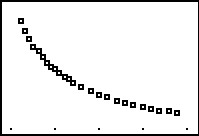
\includegraphics[width=2in]{./RationalsGraphics/Rationals15.jpg} \hspace{0.75in} & 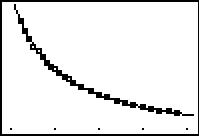
\includegraphics[width=2in]{./RationalsGraphics/Rationals16.jpg} \\

%The graph of the data  \hspace{0.75in} & The data with $y=\frac{1400}{x}$ \\


%\end{tabular}
%\end{center} 



%\item  After performing a `Power Regression', the calculator fits the data to the curve $y = ax^b$ where $a \approx 1400$ and $b \approx -1$ with a correlation coefficient which is darned near perfect.\footnote{We will revisit this example once we have developed logarithms in Chapter \ref{ExpLogs} to see how we can actually `linearize' this data and do a linear regression to obtain the same result.}  In other words, $y = 1400 x^{-1}$ or $y = \frac{1400}{x}$, as we guessed.


%\begin{center}

%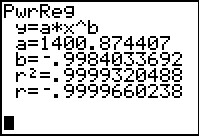
\includegraphics[width=2in]{./RationalsGraphics/Rationals17.jpg}

%\end{center} 

%\qed

%\end{enumerate}

%\end{ex}

%\newpage

\printexercises{exercises_pre/04_03_exercises}
